% author: Aditya Baradwaj
% email: abaradwaj@berkeley.edu

\qns{Projections}

\meta{
Description: Introduction to projections
}

\begin{enumerate}

\begin{center}
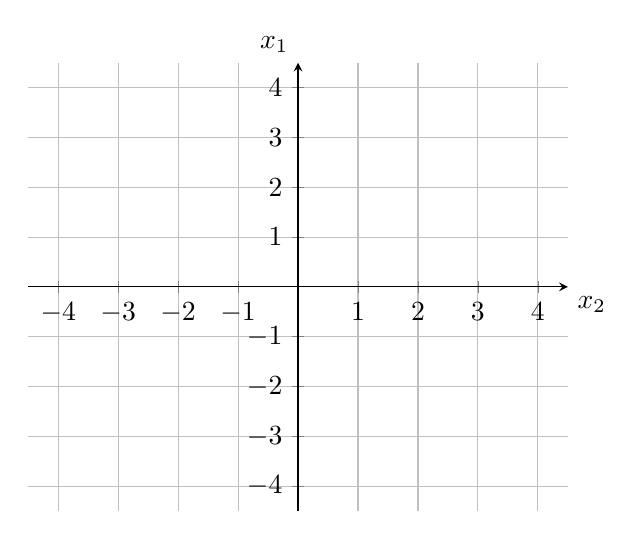
\begin{tikzpicture}[>=latex]
\begin{axis}[
  axis x line=center,
  axis y line=center,
   xtick={-4,...,4},
  ytick={-4,...,4},
  xlabel={$x_2$},
  ylabel={$x_1$},
  xlabel style={below right},
  ylabel style={above left},
  xmin=-4.5,
  xmax=4.5,
  ymin=-4.5,
  ymax=4.5,
  grid]
\end{axis}
\end{tikzpicture}
\end{center}

\qitem{
Consider the vector $\vec{x} = \begin{bmatrix}2 \\ 4\end{bmatrix}$. Draw it on the graph provided. Also draw the vectors $\vec{x}$ with the vector $\vec{y_1} = \begin{bmatrix}1 \\ 0\end{bmatrix}$ and $\vec{y_2} = \begin{bmatrix}0 \\ 1\end{bmatrix}$. Now, find the inner product of $\vec{x}$ with $\vec{y_1}$ and $\vec{y_2}$.
}

\ans{
$$\innp{x}{y_1} = 2 \cdot 1 + 4 \cdot 0 = 2$$
$$\innp{x}{y_2} = 2 \cdot 0 + 4 \cdot 1 = 4$$
}

Interestingly, we notice that the inner products of $\vec{x}$ with each of the unit vectors in the x and y directions gives us the components of the vector in those directions. This is not a coincidence. If we drop perpendiculars from the vector $\vec{x}$ to tne x and y axis, the resulting vectors are just $y_1$ and $y_2$. This 'dropping a perpendicular' is what we mean by projection.

\qitem{
Now, find the inner product of $\vec{x}$ with the vector $\vec{y_3} = \begin{bmatrix}5 \\ 0\end{bmatrix}$. Is this the same as with $\vec{y_1}$? How can we find the projection of $\vec{x}$ onto $\vec{y_3}$?
}

\ans{
$$\innp{x}{y_3} = 2 \cdot 5 + 4 \cdot 0 = 10$$
However, by dropping the perpendicular from $\vec{x}$ to $\vec{y_1}$, we can see that the projection should be the same as it was for $\vec{x_1}$. So, we have to divide this inner product by 5 to get the correct length of the projection (since $10/5 = 2$). It is not a coincidence that 5 is also the length of $\vec{x_3}$! We have to divide the inner product by the magnitude of the vector we are projecting onto, because while the inner product scales with both of its inputs, the projection should only scale with $\vec{x}$, and it should only depend on the direction of $\vec{y_3}$. That is, the projection of $\vec{x}$ onto any vector of the form $\alpha\begin{bmatrix}1 \\ 0\end{bmatrix}$ for nonzero $\alpha$ should be the same.

So, we have that the length of the projection of $\vec{x}$ onto $\vec{y}$ equals

\newcommand{\norm}{\lVert #1 \rVert}

% $\lVert hi \rVert$ blah blah blah $\norm{hi}$

 $\frac   {  \innp {\vec{x}} {\vec{y}}   }          {\norm{\vec{y}}}$.

Another way of interpreting this is that by dividing by $\norm{\vec{y}}$, we are converting $\vec{y}$ into a unit vector. That is, $\frac{\innp{\vec{x}}{\vec{y}}}{\norm{\vec{y}}} = \innp{\vec{x}}{\frac{\vec{y}}{\norm{\vec{y}}}}$
}

\qitem{
Now, let $\vec{x} = \begin{bmatrix}1 \\ 2 \\ 3\end{bmatrix}$ and $\vec{y} = \begin{bmatrix}1 \\ 0 \\ -1\end{bmatrix}$. Find the projection of $\vec{x}$ onto $\vec{y}$. Also find the projection of $\vec{y}$ onto $\vec{x}$.
}

\ans{
The length of the projection of $\vec{x}$ onto $\vec{y}$ will be $\frac{\innp{\vec{x}}{\vec{y}}}{||\vec{y}||} = \frac{1 \cdot 1 + 0 \cdot 2 + 3 \cdot -1}{\sqrt{1^2 + 0^2 + 1^2}} = \frac{-2}{\sqrt{2}} = -\sqrt{2}$.

But we don't just want the length of the projection, we want the actual projection vector. We know the projection's length, and we know that it must lie along the direction characterized by $\vec{y}$. So to get the projection, we can simply scale the unit vector in the direction of $\vec{y}$ by the length we found above.
So, the projection is $-\sqrt{2} \cdot \frac{\vec{y}}{||\vec{y}||} = -\sqrt{2} \frac{1}{\sqrt{2}} \begin{bmatrix}1 \\ 0 \\ -1\end{bmatrix} = \begin{bmatrix}-1 \\ 0 \\ 1\end{bmatrix}$.
}

\qitem{
Let $\m{A} = \begin{bmatrix}
1 & 0 & -1 \\
0 & 1 & -1 \\
1 & 1 & -1
\end{bmatrix}$
Suppose we know that $A^T\vec{x} = \vec{0}$. Based on your knowledge of inner products and projections, what does this tell you about the vector $\vec{x}$
}

\ans{
It tells you that the vector $\vec{x}$ is orthogonal to the columns of $\m{A}$. Or, in other words, the projection of $\vec{x}$ onto each of the columns of $\m{A}$ is of length 0. This also means that the projection of $\vec{x}$ onto the subspace spanned by the columns of $\m{A}$, also known as the range of $\m{A}$, is the zero vector.
}

\meta{
Draw out the column space of $\m{A}$ for the students in 3D, and indicate the direction that $\vec{x}$ would lie in.
}


\end{enumerate}
